\documentclass[12pt]{report}
\usepackage[T1]{fontenc}
\usepackage[utf8]{inputenc}
\usepackage{lmodern, textcomp} %textcomp for usage of euro currency symbol
\usepackage{listings}
\usepackage[margin=1in]{geometry}
\usepackage{csquotes}
\usepackage[english]{babel}
\usepackage{color}
\usepackage{xcolor} %for more colours to use in hyperref
\usepackage{amsmath}
\usepackage{makecell} %for resizing hline
\usepackage{float}
\usepackage{graphicx} %for pictures
\graphicspath{ {figures/} }
\usepackage[
    backend=biber,
    style=numeric,
    sorting=none
    ]{biblatex}
\addbibresource{ref.bib}

\usepackage{hyperref}
\hypersetup{
    colorlinks=true, %set true if you want colored links
    linkcolor={red!50!black},
    citecolor={blue!50!black},
    urlcolor={blue!80!black}
    }
    
\usepackage{listings}
\usepackage{color}


\usepackage{graphicx}
\usepackage{caption}
\usepackage{subcaption}

\definecolor{mygreen}{rgb}{0,0.6,0}
\definecolor{mygray}{rgb}{0.5,0.5,0.5}
\definecolor{mymauve}{rgb}{0.58,0,0.82}

\lstset{ %
  backgroundcolor=\color{white},   % choose the background color; you must add \usepackage{color} or \usepackage{xcolor}; should come as last argument
  basicstyle=\footnotesize,        % the size of the fonts that are used for the code
  breakatwhitespace=false,         % sets if automatic breaks should only happen at whitespace
  breaklines=true,                 % sets automatic line breaking
  captionpos=b,                    % sets the caption-position to bottom
  commentstyle=\color{mygreen},    % comment style
  deletekeywords={...},            % if you want to delete keywords from the given language
  escapeinside={\%*}{*)},          % if you want to add LaTeX within your code
  extendedchars=true,              % lets you use non-ASCII characters; for 8-bits encodings only, does not work with UTF-8
  frame=single,	                   % adds a frame around the code
  keepspaces=true,                 % keeps spaces in text, useful for keeping indentation of code (possibly needs columns=flexible)
  keywordstyle=\color{blue},       % keyword style
  language=Octave,                 % the language of the code
  morekeywords={*,...},           % if you want to add more keywords to the set
  numbers=left,                    % where to put the line-numbers; possible values are (none, left, right)
  numbersep=5pt,                   % how far the line-numbers are from the code
  numberstyle=\tiny\color{mygray}, % the style that is used for the line-numbers
  rulecolor=\color{black},         % if not set, the frame-color may be changed on line-breaks within not-black text (e.g. comments (green here))
  showspaces=false,                % show spaces everywhere adding particular underscores; it overrides 'showstringspaces'
  showstringspaces=false,          % underline spaces within strings only
  showtabs=false,                  % show tabs within strings adding particular underscores
  stepnumber=2,                    % the step between two line-numbers. If it's 1, each line will be numbered
  stringstyle=\color{mymauve},     % string literal style
  tabsize=2,	                   % sets default tabsize to 2 spaces
  title=\lstname                   % show the filename of files included with \lstinputlisting; also try caption instead of title
}

\usepackage{algorithm}
\usepackage[noend]{algpseudocode}
\makeatletter
\def\BState{\State\hskip-\ALG@thistlm}
\makeatother

\newcommand*\samethanks[1][\value{footnote}]{\footnotemark[#1]}

\title{\Large{\textbf{Assignment 1}}\\\Large{IEORE 4742 Deep Learning for OR and FE}}

\author{
    Ahmad Shayaan\thanks{All authors contributed equally to this work.} \\as5948
    } 

\date{
\{\href{mailto:ahmad.shayaan@columbia.edu}{\texttt{\small{ahmad.shayaan@columbia.edu}}}\}\texttt{\small{@columbia.edu}}\\
    Columbia University\\
    \today}



\usepackage[utf8]{inputenc}

% Default fixed font does not support bold face
\DeclareFixedFont{\ttb}{T1}{txtt}{bx}{n}{12} % for bold
\DeclareFixedFont{\ttm}{T1}{txtt}{m}{n}{12}  % for normal

% Custom colors
\usepackage{color}
\definecolor{deepblue}{rgb}{0,0,0.5}
\definecolor{deepred}{rgb}{0.6,0,0}
\definecolor{deepgreen}{rgb}{0,0.5,0}

\usepackage{listings}

% Python style for highlighting
\newcommand\pythonstyle{\lstset{
		language=Python,
		basicstyle=\ttm,
		otherkeywords={self},             % Add keywords here
		keywordstyle=\ttb\color{deepblue},
		emph={MyClass,__init__},          % Custom highlighting
		emphstyle=\ttb\color{deepred},    % Custom highlighting style
		stringstyle=\color{deepgreen},
		frame=tb,                         % Any extra options here
		showstringspaces=false            % 
	}}
	
	
	% Python environment
	\lstnewenvironment{python}[1][]
	{
		\pythonstyle
		\lstset{#1}
	}
	{}
	
	% Python for external files
	\newcommand\pythonexternal[2][]{{
			\pythonstyle
			\lstinputlisting[#1]{#2}}}
	
	% Python for inline
	\newcommand\pythoninline[1]{{\pythonstyle\lstinline!#1!}}

\begin{document}

\maketitle
\tableofcontents

\pagebreak

\chapter{Solution for Question 1}
\section{Question 1 Part 1}
We had to design an algorithm that linearly separates two curves defined on the space $\Omega$. Where is $\Omega = [-1,1] \times [-1,1]$ and the equation of the curves are given as follows.

\begin{equation*}
	y_1 = -0.6\sin{(\frac{\pi}{2} + 3x)} - 0.35 
\end{equation*}
\begin{equation*}
	y-2 = -0.6\sin{(\frac{\pi}{2} +3x)} + 0.25
\end{equation*}

\noindent The curve plotted in the space are shown in \figurename{\ref*{fig:1}}
\begin{figure}[H]
	\begin{center}
		\includegraphics[scale = 0.3]{"que1a_curve"}
		\caption{Curves Plotted in the space $\Omega$}
		\label{fig:1}
	\end{center}
\end{figure}

I decided to label one of the figure with class label one and the other with class label zero. I then proceeded to train a logistic regression separator with loss criteria as Binary Cross entropy loss. The implementation of the linear separator class is given below. I used python and PyTorch library to implement the linear separator.

\

\begin{python}
class LinearSperator():
	"""docstring for LinearSperator"""
	def __init__(self,learning_rate):
		self.learning_rate = learning_rate
		self.W = torch.ones(1,dtype=torch.float64,requires_grad=True)
		self.B = torch.ones(1,dtype=torch.float64,requires_grad=True)
		self.optimizer = torch.optim.SGD([self.W,self.B],lr = self.learning_rate)
		self.loss = nn.BCELoss(reduction='mean')


	def forward(self,data):
		return torch.sigmoid(self.W*data + self.B)


	def train(self,data,label):
		output = self.forward(data)
		loss = self.loss(output,label)
		print (loss.item())
		self.optimizer.zero_grad()
		loss.backward()
		self.optimizer.step()
\end{python}

\
At each iteration the model is fed in a curve and the output is then used to adjust the weights to correctly classify the curves. I used the Stochastic Gradient Descent optimizer of PyTorch library to adjust the weights. \figurename{\ref{fig:2}} shows the linear separator.

\begin{figure}[H]
	\begin{center}
		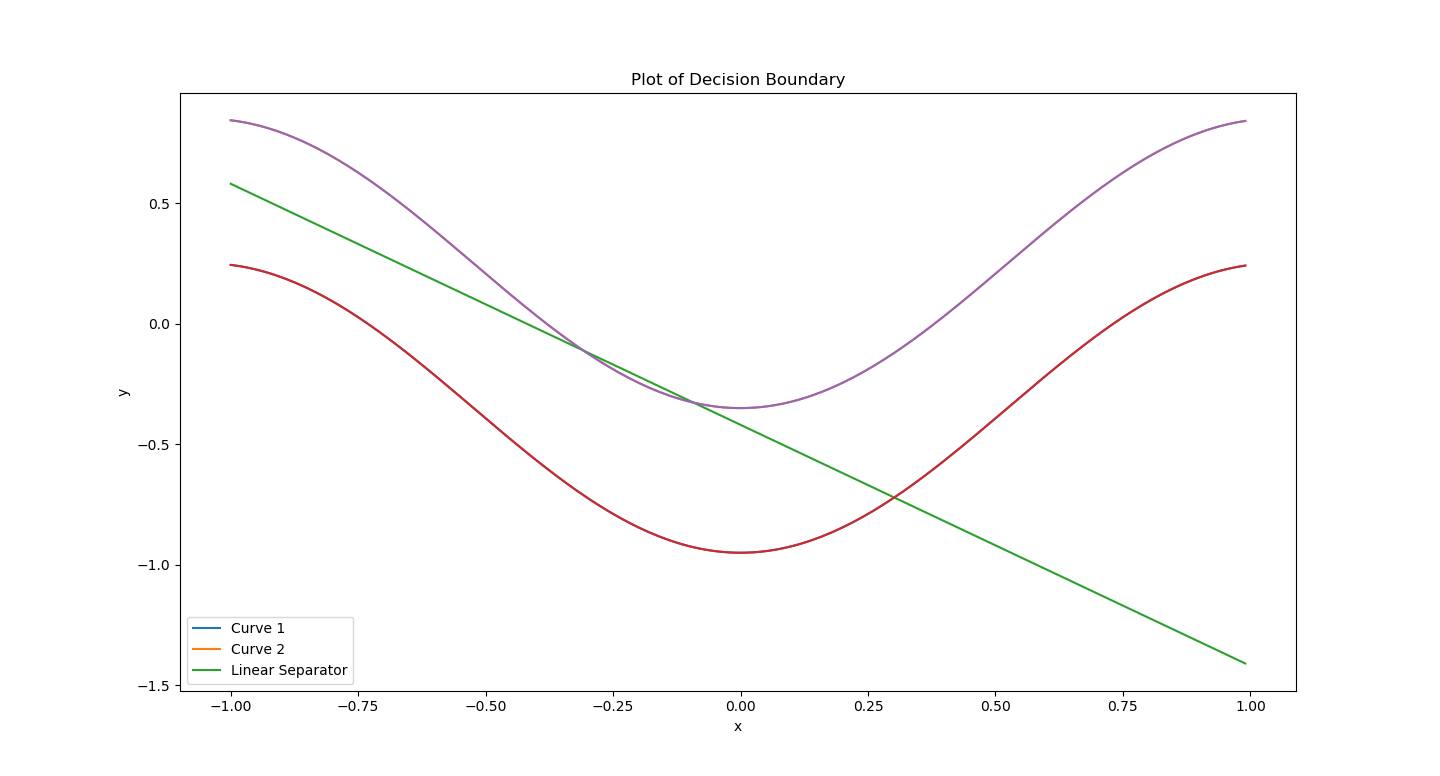
\includegraphics[scale = 0.3]{que1_seperator}
		\caption{Linear Separator for the two curves}
		\label{fig:2}
	\end{center}
\end{figure} 

 The separator almost separates the two curves in the space $\Omega$.
 
\section{Question 1 Part 2}

In this question we had to do a gird search to find the optimal parameters for the transformed space and also the parameters for the separator in the transformed space. I used a grid search approach to find the global  optimal for the set $\{W_{11},W_{12},W_{21},W_{22},b_1,b_2,a,b,c\}$ . The source code for my solution is shown below.

\

\begin{python}
	def generatingSpace():
		for w11 in range(-3,3):
			for w12 in range(-3,3):
				for w21 in range(-3,3):
					for w22 in range(-3,3):
						for b1 in range(-1,2):
							for b2 in range(-1,2):
								for a in range(-6,6):
									for b in range(-6,6):
										for c in range(-6,6):
											w = np.array([a,b,c])
											Flag = True
											
											x_hat = np.tanh(w11*x + w21*y + b1)
											y_hat = np.tanh(w12*x + w22*y + b2)
											
											x_hat_curve_1 = np.tanh(w11*x + w21*y1 + b1)
											y_hat_curve_1 = np.tanh(w12*x + w22*y1 + b2)
											
											x_hat_curve_2 = np.tanh(w11*x + w21*y2 + b1)
											y_hat_curve_2 = np.tanh(w12*x + w22*y2 + b2)
											
											for (i,j) in zip(x_hat_curve_1, y_hat_curve_1):
											product = np.dot(w, np.array([i,j,1]))
											if product >= 0:
											Flag = False
											break
											
											if Flag==True:
												for (i,j) in zip(x_hat_curve_2, y_hat_curve_2):
											
												product = np.dot(w, np.array([i,j,1]))
													if product < 0:
													Flag = False
													break
											
											if Flag==True:
												return w11, w12, w21, w22, b1, b2, a, b, c
\end{python}


\

Using grid search we are able to find the best linear separator as it enumerates over all the possible combinations in the parameter space. The Linear Separator  is shown  in \figurename{\ref{fig:3}}.

\begin{figure}[H]
	\begin{center}
		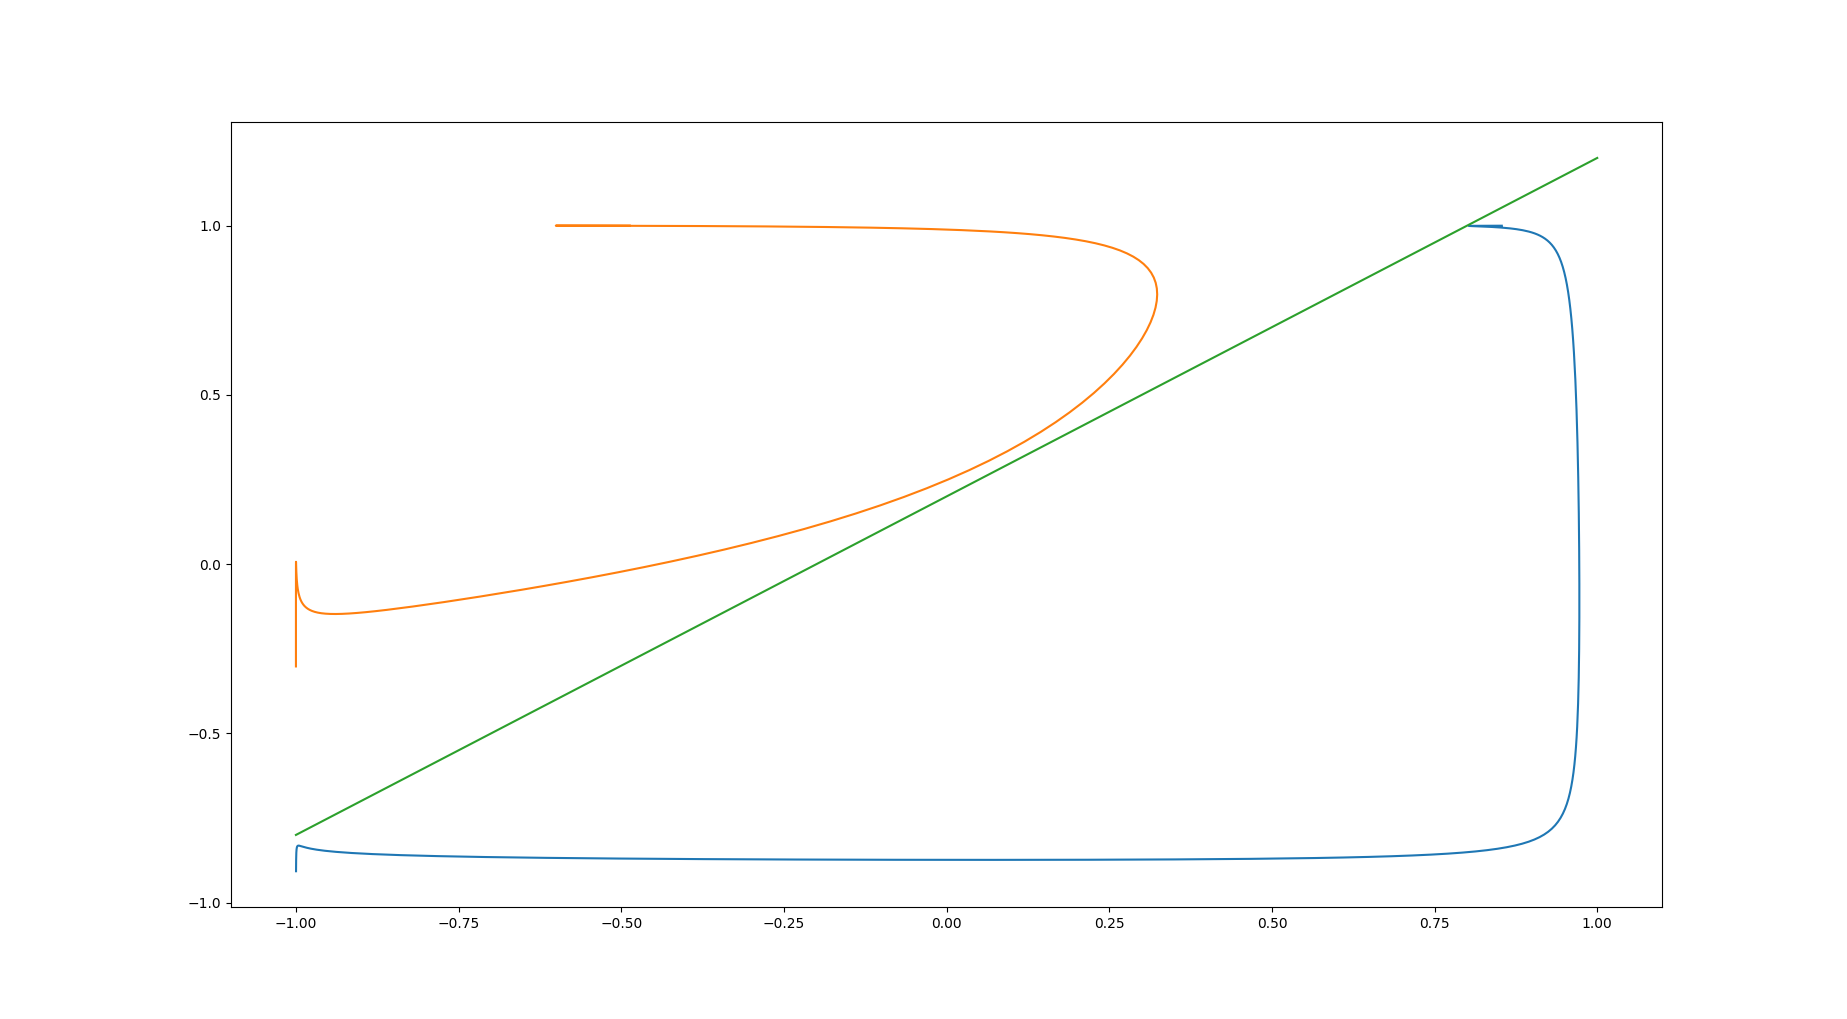
\includegraphics[scale=0.3]{que1b}
		\caption{Grid Search Linear Separator}
		\label{fig:3}
	\end{center}
\end{figure}


Table \ref{tbl:1} shows the values of the optimal parameter set obtained by gird search.

\begin{table}[H]
	\begin{center}
		\caption{Optimal Parameter Set}
		\begin{tabular}{|c|c|}
			\hline
			Parameters & Value \\ \hline
			W11        & -3    \\ \hline
			W12        & -3  \\ \hline
			W21        & -3    \\ \hline
			W22        &  2     \\ \hline
			b1         & -1    \\ \hline
			b2         &  1     \\ \hline
			a          &  -5    \\ \hline
			b          &  5     \\ \hline
			c          & -1    \\ \hline
		\end{tabular}
		
		\label{tbl:1}
	\end{center}
\end{table}

\section{Question 1 Part 2}

In this question I used other strategies to find the optimal parameter set for the transformation and the linear separator. I used logistic regression and SVM to find the optimal parameter set. I stopped searching for the optimal parameter set when the mean accuracy of classification of the two curve is above some threshold. The threshold to stop searching for the optimal parameter set was set empirically. 

The source for finding the optimal parameters sets using logistic regression and support vector machines is given below. 

\begin{python}
	def generatingSpace():
		for w11 in range(-3,4,1):
			for w12 in range(-3,4,1):
				for w21 in range(-3,4,1):
					for w22 in range(2,4,1):
						for b1 in range(0,2,1):
							for b2 in range(0,2,1):
								clf = svm.SVC(kernel='linear',gamma='auto')
								lr = LogisticRegression()
								x_hat_curve_1 = np.tanh(w11*x + w21*y1 + b1)
								y_hat_curve_1 = np.tanh(w12*x + w22*y1 + b2)
								
								x_hat_curve_2 = np.tanh(w11*x + w21*y2 + b1)
								y_hat_curve_2 = np.tanh(w12*x + w22*y2 + b2)
								
								
								x_hat = np.concatenate((x_hat_curve_1,x_hat_curve_2),axis=0)
								y_hat = np.concatenate((y_hat_curve_1,y_hat_curve_2),axis=0)	
								
								
								label1 = np.repeat(np.array([1]),x_hat_curve_1.shape[0])
								label2 = np.repeat(np.array([-1]),x_hat_curve_2.shape[0])
								labels = np.concatenate((label1,label2))
								
								df = pd.DataFrame({'X':x_hat[:],'Y':y_hat[:],'labels':labels[:]})
								df = shuffle(df)
								
								
								data = np.array([df['X'],df['Y']]).reshape(400,2)
								labels = np.array(df['labels'])
								
								clf.fit(data,labels) 
								lr.fit(data,labels)
								
								print ("SVM SCORE " + str(clf.score(data,labels)))
								print ("LR SCORE " + str(lr.score(data,labels)))
								
								if (lr.score(data,labels) > 0.57):
									return w11,w12, w21, w22, b1, b2, lr.coef_[0],lr.intercept_[0].
\end{python} 

Logistic regression seeks to minimize the cross entropy loss where as the support vector machine uses the hinge loss function in which we seek to maximize the margins from both the curve and fit the most optimal separator. Figure~\ref{fig:5} and \ref{fig:6} show the linear separators found using the two different strategies.

\begin{figure}[h]
	\begin{center}
		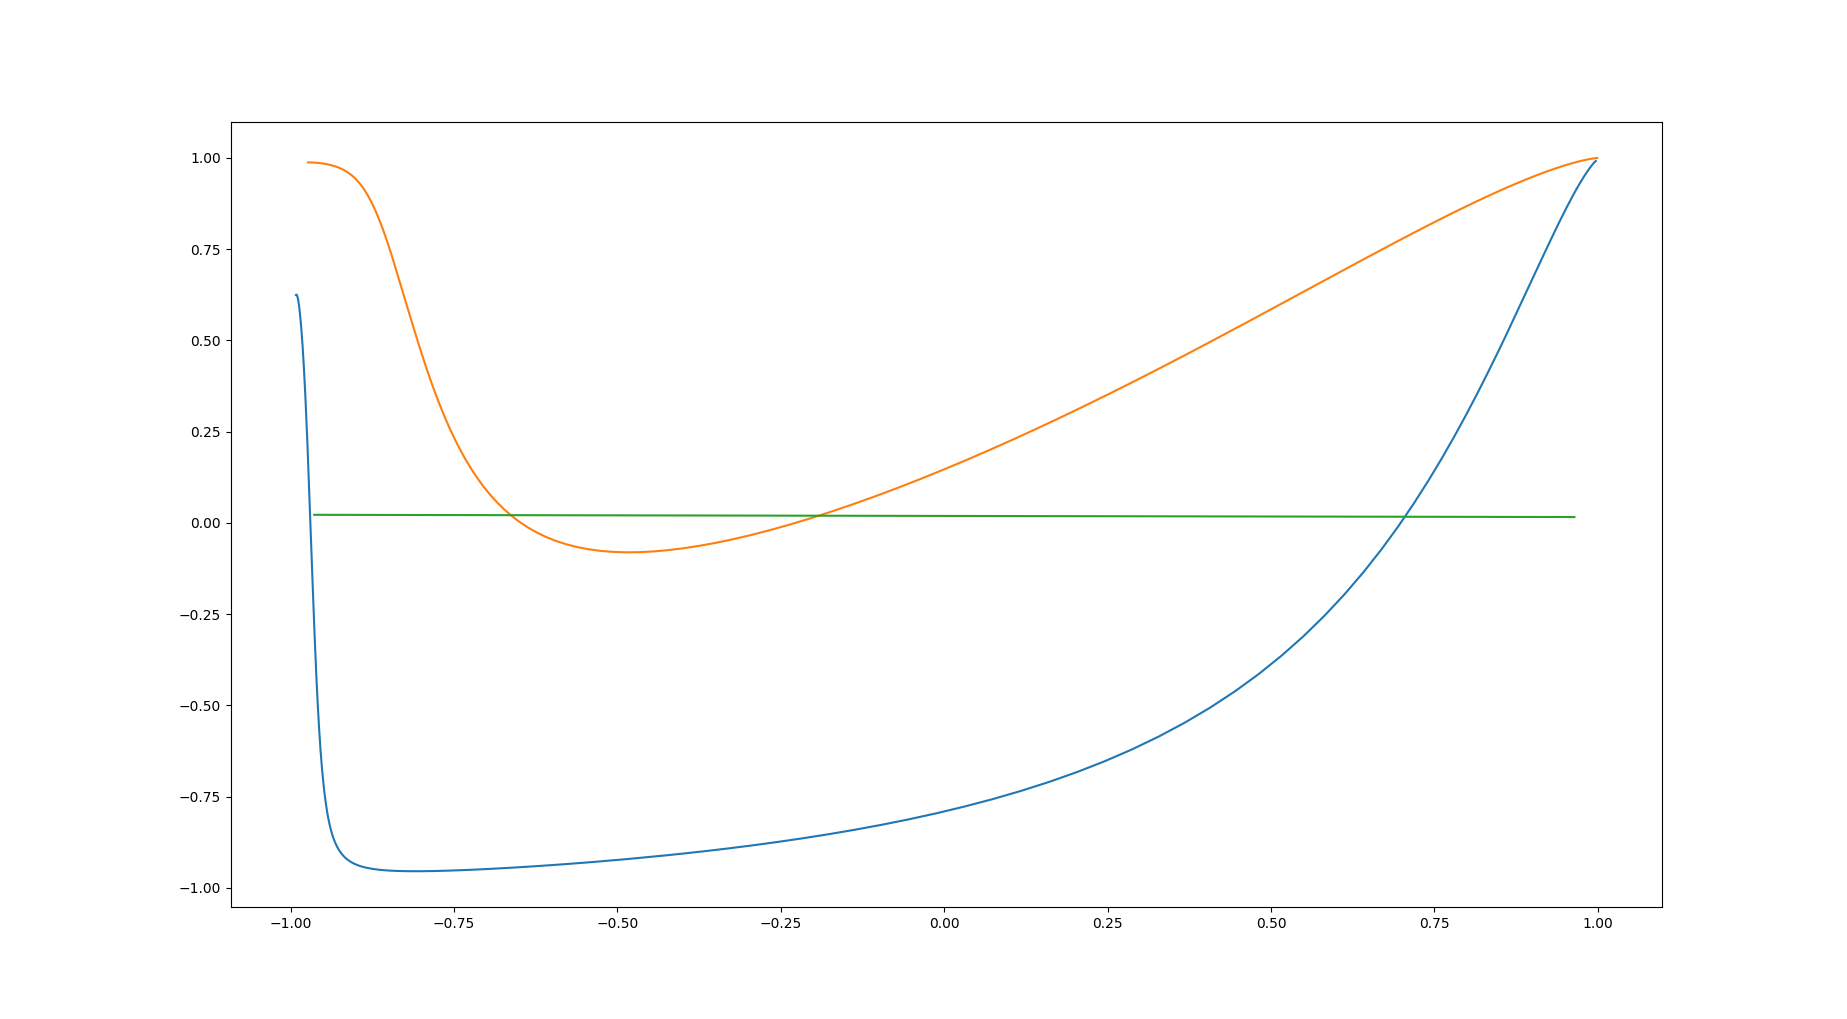
\includegraphics[scale=0.3]{que2}	
		\caption{SVM Linear separator}
		\label{fig:5}
	\end{center}
\end{figure}


\begin{figure}[h]
	\begin{center}
		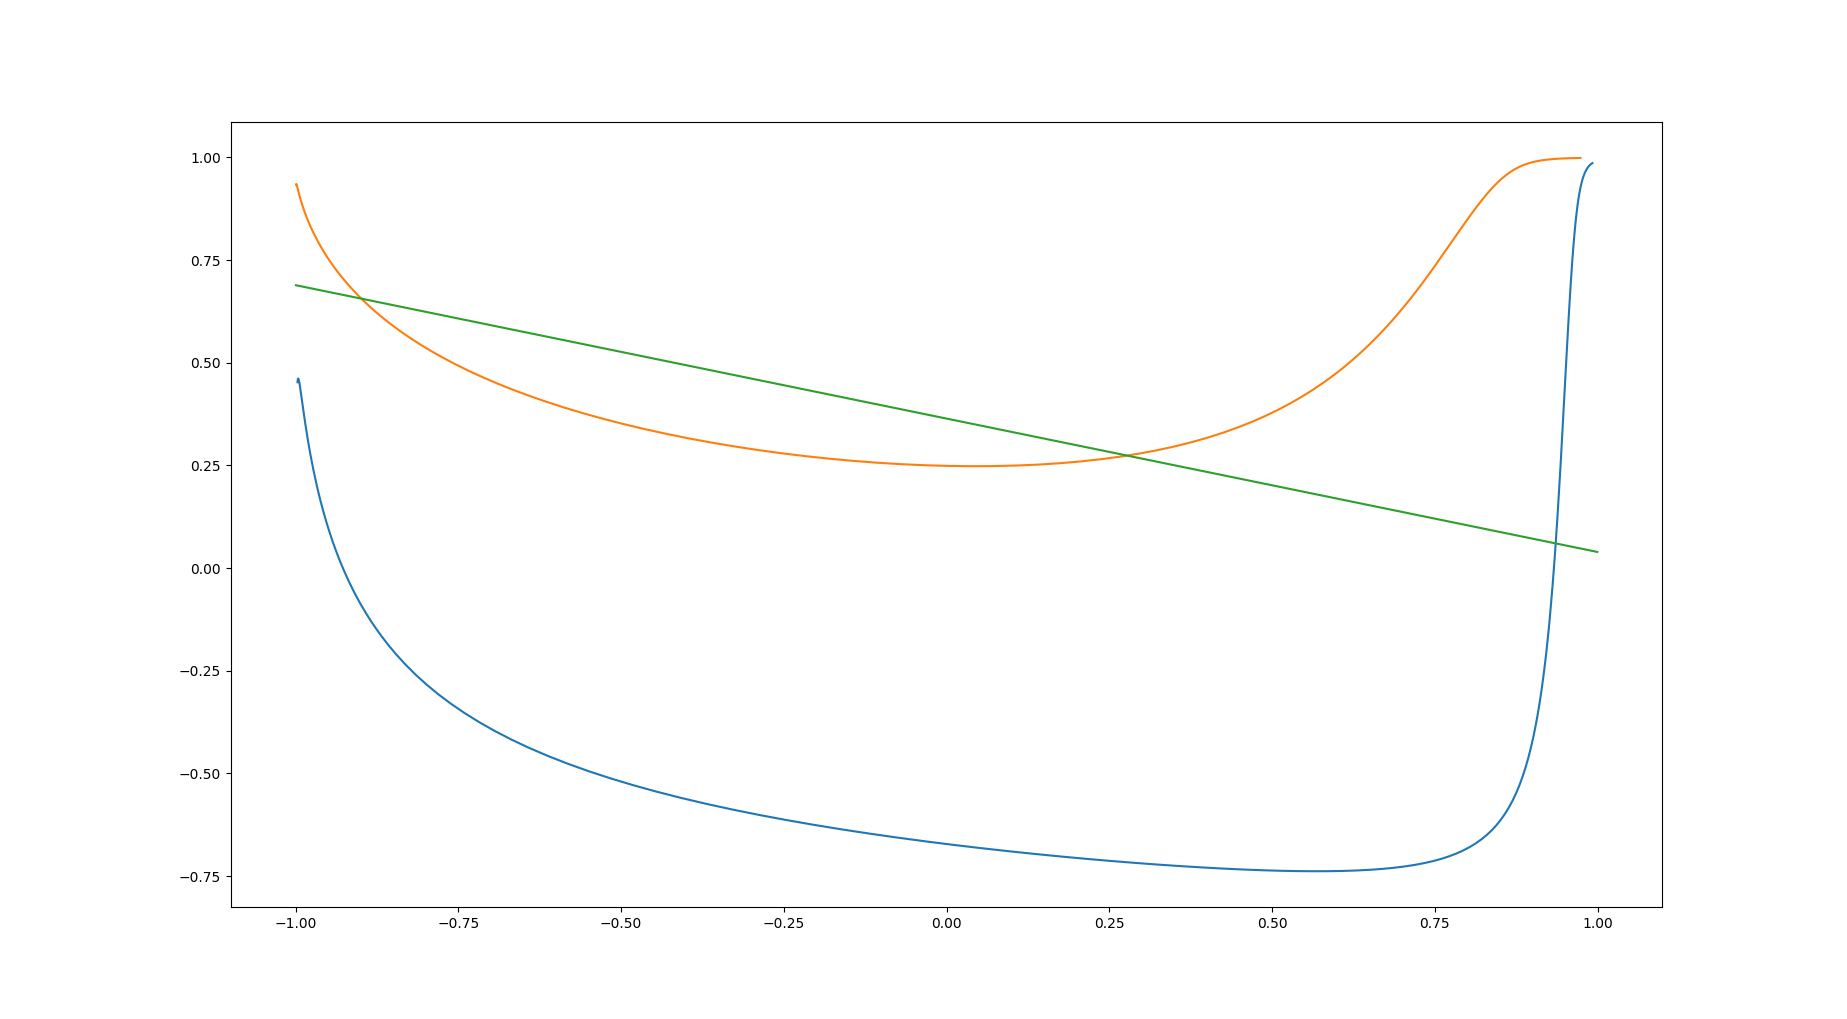
\includegraphics[scale=0.3]{que2_lr}	
		\caption{Logistic Regression Linear separator}
		\label{fig:6}
\end{center}

The linear separator are not as good as the gird search because these strategies stop when they reach a local optimum where as in grid search we stop when we reach a global optimum. The optimal parameter set found by the two strategies is shown in Table.

\begin{table}[H]
	\caption{Optimal Parameter set for LR and SVM}
	\centering
	\begin{tabular}{|c|c|c|}
		\hline
		Parameters & Logistic Regression Values & SVM Values \\ \hline
		W11        & -3                         & -3         \\ \hline
		W12        & -1                         & -2         \\ \hline
		W21        & -1                         & -2         \\ \hline
		W22        & 2                          & 3          \\ \hline
		b1         & 0                          & 0          \\ \hline
		b2         & 1                          & 1          \\ \hline
		a          & 0.12                       & -0.0096    \\ \hline
		b          & 0.369                      & 1.015      \\ \hline
		c          & -0.134                     & -0.0054    \\ \hline
	\end{tabular}
	\label{tb:2}
\end{table}

\end{figure}
	
	
\chapter{Solution for Question 2}

\section{Question 2 Part 1}

We had to plot the curves defined by the parameters given in the questions. The code to generate and plot the curves is given below. 

\begin{python}
	def generatingSpace(t):
		r1 = 50 + 0.2 * t
		r2 = 30 + 0.4 * t
		phi1 = -0.06*t + 3
		phi2 = -0.08*t + 2
		
		#curve1
		x1 = r1 * np.cos(phi1)
		y1 = r1 * np.sin(phi1)
		
		#curve2
		x2 = r2 * np.cos(phi2)
		y2 = r2 * np.sin(phi2)
		
		plt.plot(x1,y1)
		plt.plot(x2,y2)
		plt.show()
		
		return np.array([x1,y1,np.ones(x1.shape)]), np.array([x2,y2,np.zeros(x2.shape)])
\end{python}

Figure~\ref{fig:8} shows the two curves.

\begin{figure}
	\centering
	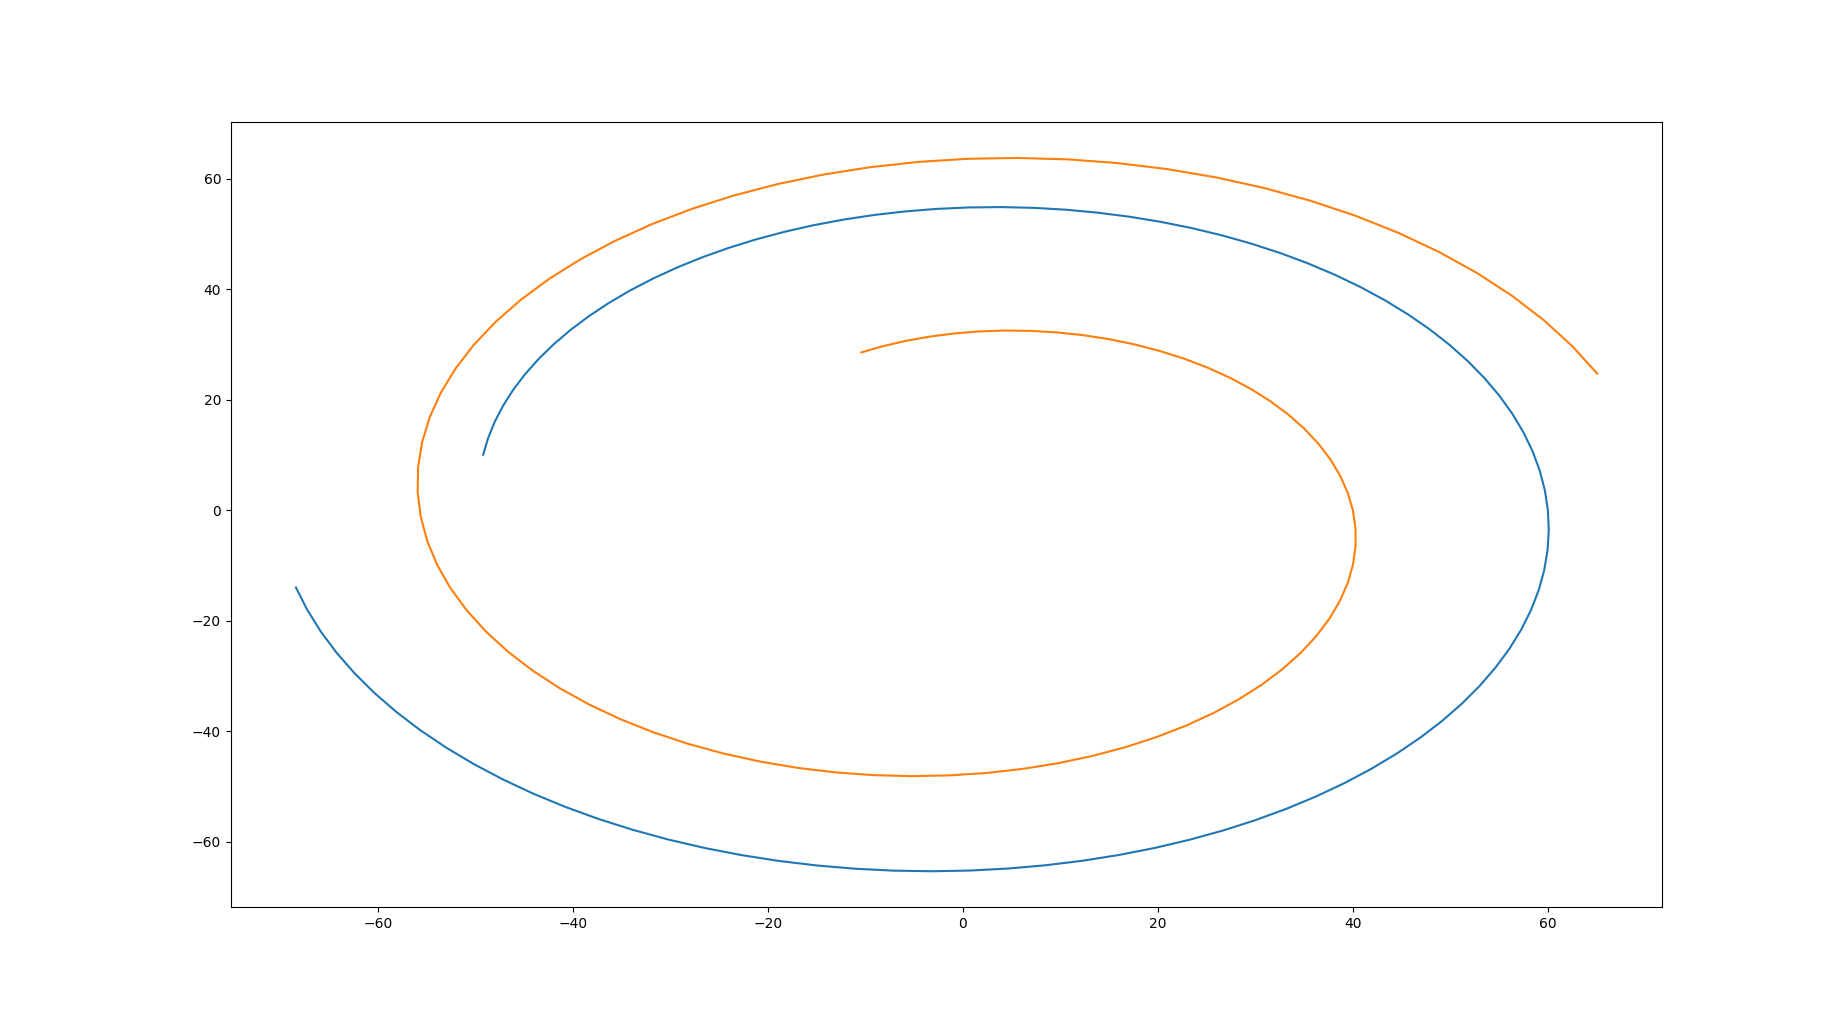
\includegraphics[scale=0.3]{question3}
	\caption{The given curves}
	\label{fig:8}
\end{figure}

\section{Question 2 Part 2}
We had to code a feed forward neural network to linear classification of the given curves. I used python to code the neural network. My solution consisted of two parts. I used the neural network to transform the topology of the curves and then trained a linear classifier to classify the curves in the transformed space. The Class which defines the neural network and all it's parameters is shown below.

\begin{python}
	import torch
	import torch.nn as nn
	import pandas as pd
	import numpy as np
	
	class Network(nn.Module):
		"""docstring for Network"""
			def __init__(self):
			super(Network, self).__init__()
			self.relu = nn.ReLU()
			self.Sigmoid = nn.Sigmoid()
			
			self.fc1 = nn.Linear(2,12)
			self.fc2 = nn.Linear(12,18)
			self.fc3 = nn.Linear(18,8)
			self.fc4 = nn.Linear(8,4)
			self.fc5 = nn.Linear(4,2)
		
		def forward(self,data):
			out = self.relu(self.fc1(data))
			out = self.relu(self.fc2(out))
			out = self.relu(self.fc3(out))
			out = self.relu(self.fc4(out))
			out = self.relu(self.fc5(out))
			return out
\end{python}

The code to train the neural network and the linear separator is given below. I used the adam optimizer provided by the PyTorch library to find the optimal. The linear separator and the weights of the neural network are adjusted by computing the binary cross entropy loss in classification

\

\begin{python}
	class Train(object):
		"""docstring for Train"""
		def __init__(self,epochs,learning_rate):
			super(Train, self).__init__()
			self.learning_rate = learning_rate
			self.net = Network()
			self.W = torch.ones(2,requires_grad=True)
			self.b = torch.ones(1,requires_grad=True)
			self.optimizer = torch.optim.Adam(itertools.chain(self.net.parameters(), [self.W], [self.b]), lr = self.learning_rate)
			self.loss_function =  torch.nn.BCELoss(reduction='mean')
			
	def trainModel(model,df):
		total_loss = 0
		for i in range(len(df)):
		data = torch.tensor((df.iloc[i]['X'],df.iloc[i]['Y'])).float()
		label = torch.tensor(df.iloc[i]['label'])
		out = model.net.forward(data)
		out = torch.sigmoid(torch.matmul(model.W,out) + model.b )
		loss = model.loss_function(out,label)
		
		model.optimizer.zero_grad()
		loss.backward()
		model.optimizer.step()
		
		total_loss += loss.item()
		
		return model,total_loss/len(df)
\end{python}

\begin{figure}[H]
	\centering
	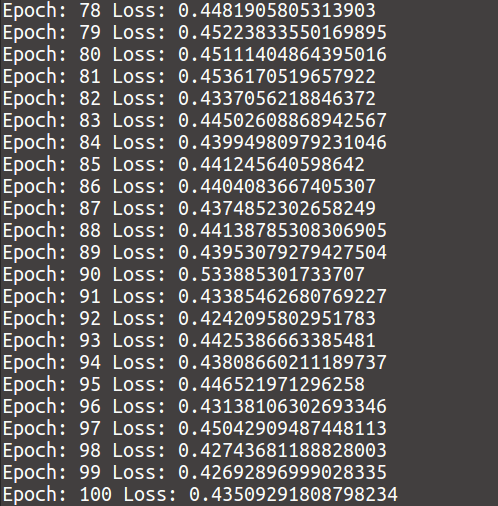
\includegraphics[scale=0.5]{que3_loss}
	\caption{Loss per epoch}
\end{figure}
The minimum loss that we attain is 0.4269.


\chapter{Solution for Question 3}
To show neural network with linear activation is with many layer is equivalent to linear neural neural network with no hidden layer.
\

\noindent Proof.	

\
Let a output of a feed forward network with n layers and activation function $\sigma_i$ at the $i^{th}$ layer be given by 
\begin{equation*} \label{eq1}
	\begin{split}
	Network & = W_n(\sigma_n(W_{n-1}(\sigma_{n-2} \dots (W_2(\sigma_1(W_1*X + b_1) )+b_2) \dots )) \\
	\end{split}
\end{equation*}

give that $\sigma(x) = x$

\begin{equation*}
\begin{split}
Network & = W_n((W_{n-1}(\dots (W_2((W_1*X + b_1) )+b_2) \dots )) \\
\end{split}
\end{equation*}

The product of all the weights can be written as written as a single weight i.e. $\Pi_i^n W_i = W$ and similarly the product of the weights and biases can be replaced by a single bias i.e. $\Pi_{i=2}^n W_i \times b_{i-1} = B$. Therefore we can write.

\begin{equation*}
	\begin{split}
		W_n((W_{n-1}(\dots (W_2((W_1*X + b_1) )+b_2) \dots )) & = WX + B \\
		Network &= WX + B 
	\end{split}
\end{equation*}

That is the network can be treated as a linear neural neural network with no hidden layer.

\end{document}